\documentclass[12pt]{IET02}
\usepackage{amsmath,amssymb}

%% Uncomment below line (note epsf package) and comment 
%% above line if using EPS figures - then use LaTeX --> DVI to PDF.
%% else, the template compiles straight using PDFLaTeX --> PDF
%\usepackage{amsmath,amssymb,epsf}

%% Load graphicx package
\usepackage{mathptmx,graphicx}
\usepackage[font=small]{subfig}

\graphicspath{{images/}}

\begin{document}

\title{Towards More Reliable and Cost Effective \\Superconducting Generators for Wind Turbines}

\markboth{O. Keysan, P. Radyjowski, J. Burchell, M. A. Mueller}{Towards More Reliable and Cost Effective uperconducting Generators for Wind Turbines}

\author{O. Keysan$^{*}$, P. Radyjowski, J. Burchell, M. A. Mueller}

\address{\textit{Institute for Energy Systems, University of Edinburgh, United Kingdom}\\
$^{*}$\textit{Email: o.keysan@ed.ac.uk}}

\keyword{superconducting generators, direct-drive, offshore wind turbines}

%\begin{abstract}
%\end{abstract}

\twocolumn

\maketitle

\section*{Abstract}
Larger offshore wind turbines help to reduce the installation and maintenance cost per unit energy generated. However, tower-head mass becomes a real challenge with conventional power take-off systems as the power rating is increased. Direct-drive superconducting generators are proposed to overcome this issue. There are many 10 MW, 10 rpm superconducting generator designs, most of which having the same topology: a synchronous machine with a conventional copper armature winding and a superconducting rotor. However, this design may not be the most suitable topology for an offshore wind turbine application, where the O&M costs are very high. 
The rotating superconducting field windings in this type of machines require rotating transfer couplings to transfer the cooling gas and they also need brushes or brushless exciters, which remains as the single point of failure in the machine, decreasing the overall reliability. Furthermore, in these designs the electromagnetic forces act on the superconducting windings, which makes the structural and thermal design challenging.
The cost of the power take-off system for a wind turbine is also very critical, and the cost of a superconducting machine is usually dominated by the cost of superconducting tape. In the common designs, the superconducting tape requirement is usually in the order of hundreds of kilometres because of two main factors: the superconducting field winding can be air-cored, which increases the MMF requirements. Secondly, even if the machine is iron-cored, the main flux path has to cross the insulation layers, vacuum and cryostat walls, which increases the equivalent magnetic gap, even if the mechanical gap is kept minimum.
In this paper, a novel transverse flux superconducting machine topology that can overcome these issues will be presented. The machine has stationary superconducting field windings and a modular claw-pole rotor. The field winding is also modular and can be placed in independent cryostat sections. Thus, even in one of the cryostat section fails machine, the machine can still operate at partial load until the maintenance. Having smaller cryostat sections also have logistics advantages such as easy installation/ transportation, and using on-site crane for any replacements. Another advantage of the topology is the minimum superconducting wire requirement. A 10 MW design is estimated to use just 15 km of MgB2 wire at 30 K. This is due to iron-cored structure and because main flux path does not cross through the cryostat (i.e. magnetic gap equals to the mechanical gap) which minimizes the required MMF.
A small linear prototype with copper winding is manufactured to prove the concept and it is planned to replace the copper winding with a high-temperature superconducting winding and repeat the tests with a proper superconducting coil at 30 K. The results will be presented in the full paper.
\vspace{1pc}

\section{Introduction}

Many superconducting machines have been designed and manufactured since the early days of superconductivity. For example, General Electric developed a 20 MW low-temperature superconducting generator in 1981 (see Fig. \ref{GE_LTS_machine}). There are a few other projects as listed in \cite{Barnes2005}, however, most of them just remained as prototypes due to cooling issues and high cost.

One of the practical applications of the superconducting machines is ship propulsion motors. Superconducting propulsion motors offer reduced mass and volume, which increases the cargo capacity or extends the range of the ship. An example of such a motor is presented in Fig. \ref{converteam_5MW}, which is manufactured by Converteam and AMSC in 2011. It can be seen from the figure that the HTS motor is twice as powerful as the load motor, it is much smaller. A 36.5 MW, 120 rpm superconducting machine was also manufactured, which weights just 75 tonnes \citep{Gamble2011}.

  \begin{figure}[]
    \centering
    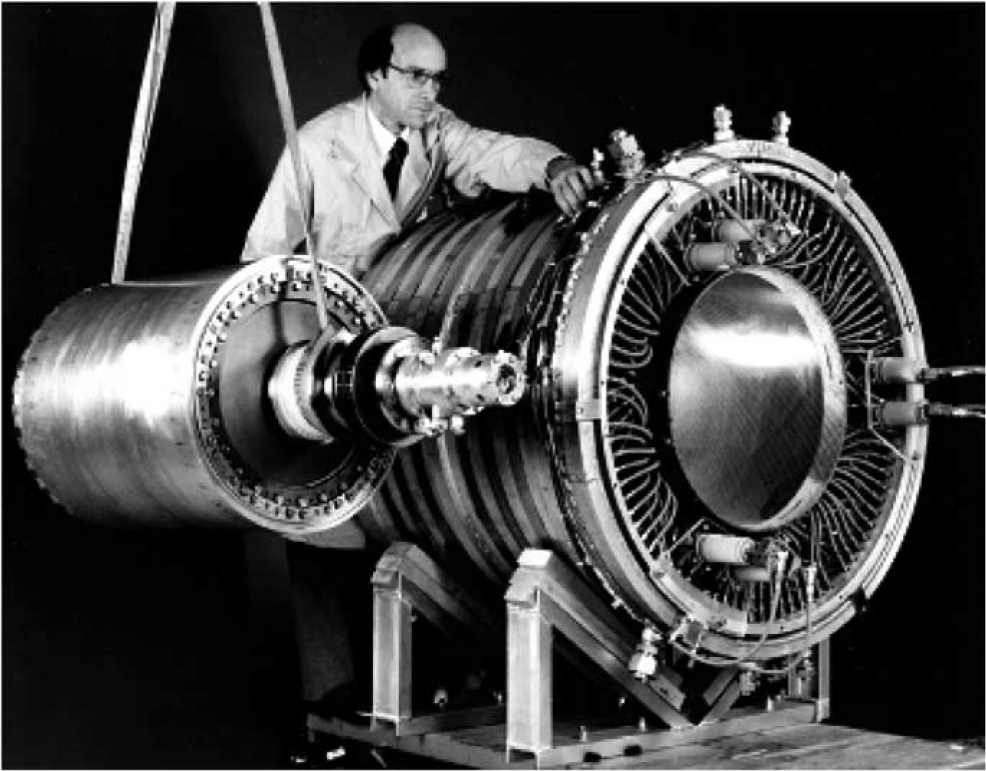
\includegraphics[width=0.3\textwidth]{GE_LTS_machine}
    \caption{General Electric's 20 MW low-temperature superconducting generator with Nb-Ti wire (1981) \cite{Barnes2005}.} 
    \label{GE_LTS_machine}
  \end{figure}

  \begin{figure}[]
    \centering
    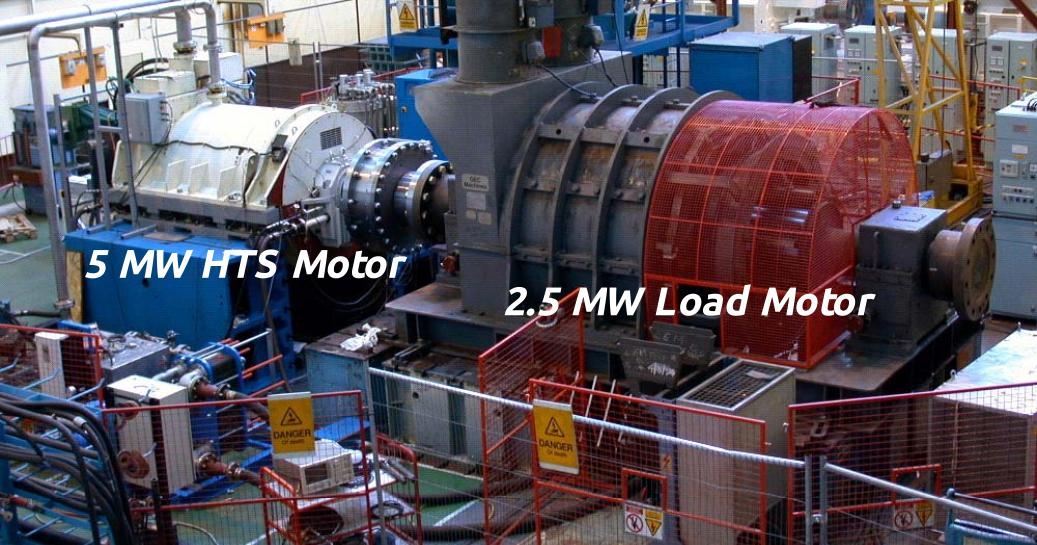
\includegraphics[width=0.45\textwidth]{converteam_5MW}
    \caption{Converteam 5 MW HTS ship propulsion motor coupled to test machine  \cite{Kalsi2004h}.} 
    \label{converteam_5MW}
  \end{figure}

The machines presented in the previous paragraph and many others have the same topology: synchronous motor with superconducting rotor. Copper windings are usually used in the armature because of AC losses in a superconducting coil limits the current density. 


Average size of onshore wind turbines are limited in 3--3.5~MW range due to transportation limitations and wind speeds. However, there is a trends towards larger wind turbines for offshore installations. This trend can be seen in Fig. \ref{offshore-turbine-size}, which shows the turbine size increased from 2 MW to 6 MW in ten years. Larger wind turbines reduces the installation and maintenance cost per MW, benefit from higher wind speeds. In \cite{Abrahamsen2010}, it is stated that 10 MW offshore wind turbines are desirable in 2020. This is a ambitious challenge to achieve with the existing power take-off(PTO) systems. The geared systems, which is the most common PTO system, have some reliability issues and the mass of the gearbox increases enormously with increasing torque requirements. Direct-drive permanent magnet generators (DDPMG) also suffer from high mass problem and the diameter of these machines are quite large. 

Superconducting machines are proposed to minimize the mass of the PTO system. The reduction of the tower head-mass will also help to reduce cost of installation and structural components costs (e.g. tower, foundation).

\begin{figure}[]
  \centering
  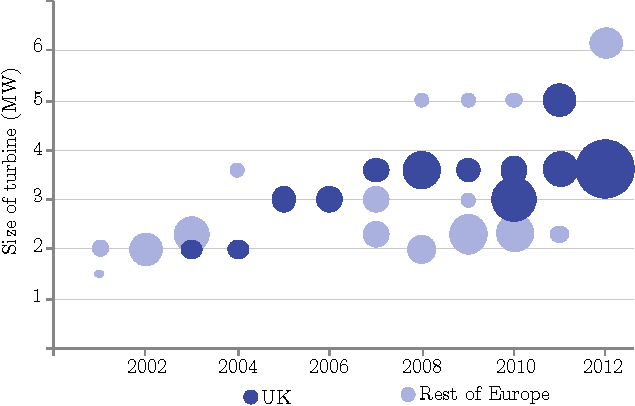
\includegraphics[width=0.45\textwidth]{offshore-turbine-size}
\caption{Commercial offshore wind farms turbine size for UK and Europe. Bubble size is proportional to the wind farm rated output \cite{bvg}.}
  \label{offshore-turbine-size}
\end{figure}





\section{A Review of Superconducting Machines}

bi onceki sectiondan devam

The synchronous generator with a superconducting rotor introduces many problems. Some of these can be listed as:

\begin{itemize}
  \item Rotating TransNo rotating transfer coupler, more robust and cheaper cooling system.
  \item No electrical brushes or complex excitation systems.
  \item No centrifugal forces and transient torques that can damage the superconducting material.
  \item Simpler winding support.
\end{itemize}

\begin{description}
  \item[Rotating Transfer Coupler:] A coupler is required to transfer the coolant from cryocoolers to the rotating superconducting coil. This coupler introduces reliability issues and requires regular maintenance. Furthermore, it is the single point of failure for the whole system. There are some designs that aim to simplify or remove the cryocoupler. For example AMSC plans to put the cold heads in the rotor for their 10 MW, 10 rpm generator design \cite{amsc_presentation}, but the design still requires couplers. General Electric plans to eliminate the cryocoupler by using a stationary superconducting coil and a rotating armature structure \cite{Stautner2012}. However, the design still requires high current electrical brushes, which require regular maintenance.

  \item[Electric Excitation System:] Brushed or brushless excitation system is required for rotating superconducting field windings.

  \item[Torque Transfer Structure:] Electromagnetic torque is generated on the superconducting winding in the conventional superconducting machine topology. Thus, it is required to design a torque transfer tube that extends through cryogenic temperature to room temperature. Usually carbon fibre materials are used to minimize the heat loss, but design of these components are difficult and increases the cost.

  \item[Transient forces in SC coil:] In a rotating superconducting winding, superconducting tape is exposed to centrifugal and other transient forces. However, second generation HTS tapes are in crystal structure and high stresses in the coil may result in cracks, which spoils the superconductivity.
\end{description}

There are also other types of superconducting machines. Instead of a superconducting field winding, magnetised bulk superconducting materials can be used, which is similar to a permanent magnet generator. Bulk superconductors can be magnetized in situ or externally. External magnetization is not a feasible method since it would be extremely difficult to handle the pre-magnetized bulk superconductors during the machine assembly. Moreover, if the cooling system fails,  the superconducting magnets will de-magnetize and the machine will be required to be disassembled.  
Thus, in situ magnetization method is the only feasible method for superconducting machines. 
In \cite{Matsuzaki2007}, HTS bulk magnets are magnetized by the pulsed field magnetization method by using a pair of the armature coils. However, the maximum flux density magnitude is limited by the current density of armature coils. There are some novel flux pumping methods that magnetize superconductors gradually by magnetic flux or thermal waves such as \cite{Masson2007b,Coombs2009}. Although these methods have some great potential, they are not proven for large scale applications yet.

There is also fully superconducting machines. Although, MgB2 wires look promising, the AC losses in the superconducting coils limits the operation frequency of such machines. A 10 MW, 10 rpm fully superconducting machine is presented in \cite{Terao2012}, but it requires 250--300~km of HTS tape and MgB2 wire each, which makes the design economically infeasible.

\section{Requirements of a Wind Turbine Generator}

There are many direct-drive superconducting generator designs for large offshore wind turbines, most of which are 10 MW, 10 rpm generators. Designers usually concentrate on electromagnetic optimization, and performance of the machine, but neglects the operating conditions and requirements of an offshore wind turbine. These can be listed as follows:

\begin{description}
  \item[\textbf{Reliability:}] The maintenance of offshore wind turbines are very difficult and expensive. Furthermore, access to the turbine is subject to the weather and the sea conditions, which adds weeks or months of lost generation income on top of the repair cost. Thus, the reliability of an offshore wind turbine is very important. The reliability of superconducting machines is questionable, but the reliability can be improved by minimising extra equipments and moving parts (such as cryocouplers or electric brushes). 

  \item[\textbf{Redundancy:}] There are some subsystems that can not be eliminated in a superconducting machine, such as the refrigeration system. In this case, redundancy should be introduced, in a way that any failures between planned maintenance periods should not cause any down times.

  \item[\textbf{Modularity:}] Modularity is another form of redundancy. Modularity has two advantages: firstly, even if a section of a PTO system fails the remaining sections can operate at partial load until the next maintenance. For example, Clipper Wind developed a wind turbine (C93 Liberty) that has four parallel PM generators coupled to the gearbox. Thus, a failure in one of the generators will only result in 25 \% loss in the power output. Secondly, by modularity each section will be kept in manageable sizes, and can be replaced by on-site cranes without the need for expensive cranes. It is stated in \cite{Kaiser2007} that the replacement of a gearbox (of an onshore wind turbine) can cost as much as 10 \% of the initial construction cost of a turbine. It is a much difficult and expensive task to replace gearbox or drive-drive generator for an offshore wind turbine.

  \item[\textbf{Tower Head Mass:}] A lower tower head mass help to reduce the installation cost and also manufacturing cost by reducing the structural mass requirements of the turbine. In the design of superconducting machines, the active material mass is usually optimised, but the structural mass is neglected. However, due to increased airgap flux densities, the stress acting on the generator structure is higher and optimisation in the structure will help to reduce the overall generator mass.

 \end{description}


\section{Proposed Generator} % (fold)
\label{sec:proposed_generator}

A transverse flux superconducting machine topology was proposed in \cite{Keysan2011e,Keysan2012a}. The generator consists of a single loop-shaped stationary superconducting coil, a modular rotor that consists of claw-poles made of laminated steel (see Fig. \ref{rotational_claw_schematic}). The biggest advantages of the design is having a stationary superconducting coil and armature. The initial design has unbalanced forces acting on the claw pole rotor and also requires use of soft magnetic composite (SMC) material in the inner stator. Thus, it is not really suitable for a large scale applications.

The machine presented in Fig. \ref{rotational_claw_side} can be rotated 90 degrees to obtain an axial flux machine as shown in Fig. \ref{axial_claw_pole}. Then, two axial machine claw poles machines can be combined to obtain a double-sided machine as shown in Fig. \ref{double_claw_pole}. In this configuration, there is also a single superconducting field winding, but the design has two independent armature windings. The magnetic flux travels along the claw poles and links the independent armature windings on each end. The magnetic attraction forces acting on the claw pole are symmetrical and cancel each other (assuming the air-gap clearance on each side is equal). 

In the double-claw machine, soft-magnetic composite material is no longer needed as the flux through the field core travels only in the axial direction, and the field core can be manufactured from steel laminations.
The advantages of the double-sided claw pole topology can be summarised as:

\begin{itemize}
  \item Stationary superconducting field winding (no transfer couplers).
  \item No electromagnetic forces acting on the superconducting coil (simpler mechanical support).
  \item Magnetic attraction forces on the large claw poles are symmetrical and cancel each other (reduced structural mass).
  \item Two independent armature windings (improved modularity).
\end{itemize}




\begin{figure}[]
  \centering
  \subfloat[Side view.]{\label{rotational_claw_side}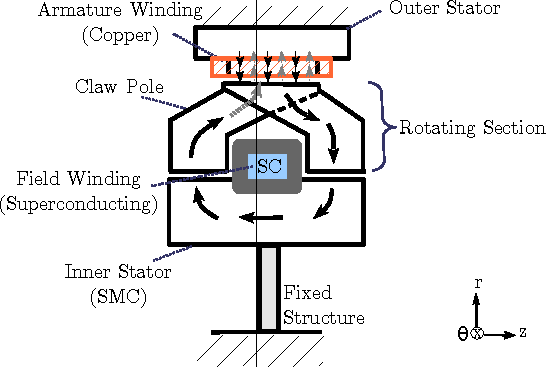
\includegraphics[scale=0.7]{rotational_claw_schematic}}

  \subfloat[Front section view.]{\label{rotational_claw_front}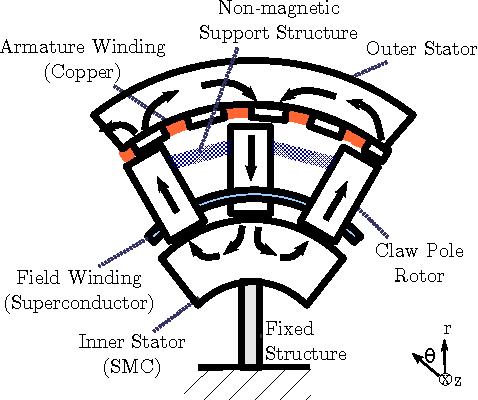
\includegraphics[scale=0.7]{rotational_claw_schematic2}}
    \caption{Basic schematic and flux lines in the transverse flux claw pole superconducting machine.} 
    \label{rotational_claw_schematic}
\end{figure}


\begin{figure}[]
  \centering
  \subfloat[Axial claw pole.]{\label{axial_claw_pole}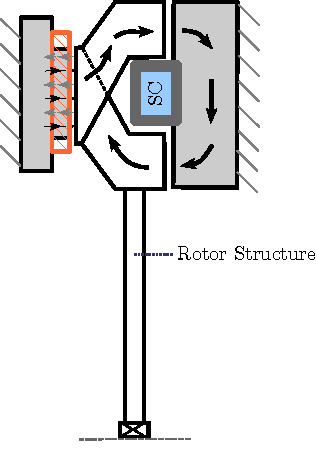
\includegraphics[scale=0.66]{axial_claw_pole}}
  \subfloat[Double-sided claw pole.]{\label{double_claw_pole}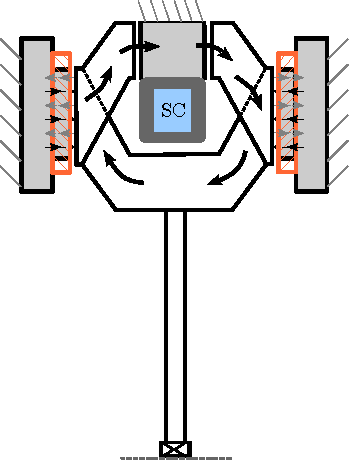
\includegraphics[scale=0.7]{double_claw_pole}}
    \caption{Evolution of the double sided transverse flux claw pole topology.} 
    \label{claw_pole_evolution}
\end{figure}

% section proposed_generator (end)

\section{Manuscript preparation}

Full papers must be typed in English. This instruction page is an
example of the format and font sizes to be used.

The title of the paper is typed in sentence case (bold 18pt) and
centred on the page. The author's initials and surname are typed
in title case bold letters and centred on the page. Directly under
the author's name in title case letters and also centred is the
author's affiliation, address, plus email address of (at least)
the corresponding author. Manuscripts must be typed single spaced
using 10 point characters. Only Times, Times Roman, Times New
Roman and Symbol fonts are accepted. The text must fall within a
frame of $18\,\hbox{cm} \times 24\,\hbox{cm}$ centred on an A4
page $(21\,\hbox{cm} \times 29.7\,\hbox{cm})$. Paragraphs are
separated by 6 points and with no indentation. The text of the
full papers is written in two columns and justified. Each column
has a width of 8.8\,cm and the columns are separated by a margin
of 0.4\,cm. Your paper must adhere to the length stipulated on the
event website. Pages should be numbered centrally at the bottom of
the page.

\subsection{\it Figures and tables}

Figures and tables should be centred in the column, numbered
consecutively throughout the text, and each should have a caption
underneath it (see for example Table 1). Care should be taken that
the lettering is not too small. All figures and tables should be
included in the electronic versions of the full paper.

\begin{table}[h]%1
\processtable{This is an example of a table caption}
{\begin{tabular}{@{}|@{\ \ \qquad}l@{\ \ \qquad}|@{\ \ \qquad}c@{\ \ \qquad}|@{}}\hline
 &\\[-.6pc]
$n$ &$n$! \\[-.6pc]
 &\\\hline
 &\\[-.6pc]
1 &1\\[-.6pc]
 &\\\hline
 &\\[-.6pc]
2 &2\\[-.6pc]
 &\\\hline
 &\\[-.6pc]
3 &3\\[.2pc]\hline
\end{tabular}}{}
\end{table}

\subsection{\it Equations}

Equations should be typed within the text, centred, and should be numbered
consecutively throughout the text. They should be referred to in the text as
Equation~(n). Their numbers should be typed in parentheses, flush right, as
in the following example.
\begin{equation}
PA + A'P - PBR^{-1}B'P + Q = 0.
\end{equation}

\section{Final PDF file}

The final format in which the papers will appear in the Proceedings will be
a PDF file. Authors are requested to send a PDF file of their final paper to
be included directly in the Proceedings. Do not lock your PDF file -- this
may result in your paper not being published.

\section{Submission of the full paper}

Your full paper should be submitted online via the conference website. It
should be expected that after your submission, your final paper will be
published directly from the PDF you send without any further proof-reading.
Therefore, it is advisable for the authors to print a hard copy of their
final version and read it carefully.

\section*{Acknowledgements}

The acknowledgement for funding organisations etc. should be placed in a
separate section at the end of the text.

Thank you for your cooperation in complying with these instructions.

\bibliography{pemd-2014}

\bibliographystyle{plain}

% \begin{thebibliography}{9}
% \vspace{1pc}

% \bibitem{}A. B. Author, C. D. Author. ``Title of the article'',
% \textit{The Journal}, \textbf{volume}, pp.~110--120, (2000).\vspace{.4pc}
% \end{thebibliography}


\end{document}
